\section{Wave-Particle Duality}
\subsection{Photoelectric Effect}
The photoelectric effect was one of a few experiments that began suggesting otherwise. The experimental set-up for studying the photoelectric effect is shown. 
\begin{figure}[ht]
\centering
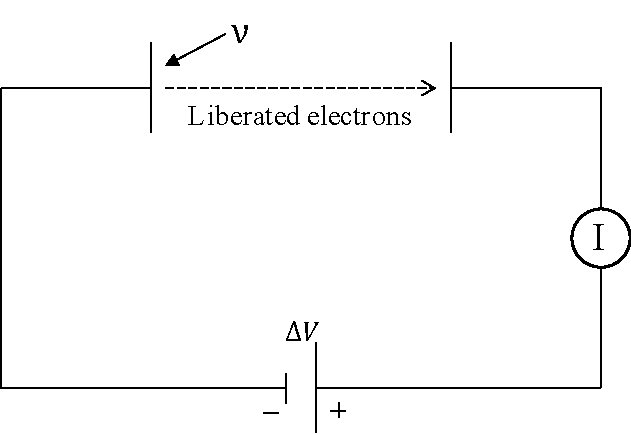
\includegraphics[width=100mm]{images/quantum/photoelectric.pdf}
\end{figure}

Light is shone upon a metallic cathode. Under certain conditions, the light is able to liberate free electrons from the metal. Electrons with enough energy are able to reach the anode, causing a current to flow. The voltage between the anode and cathode can be varied to increase or reduce this current. If we increase the voltage until no electrons make it to the anode, we can empirically measure the maximum kinetic energy of the electrons emitted.

Classically, we expect this maximum kinetic energy to increase as the intensity $I$ of the light increases. This is because we expect a more intense beam to make the electrons liberated by the beam more energetic, since intensity is power delivered per unit area. We also predict that the maximum kinetic energy to be independent of the frequency $\nu$ of the light, since frequency classically has no effect on the energy carried by the wave.

Experimentally, however, we find that the maximum kinetic energy of the electrons is fully independent of the intensity. We also see that it varies linearly with $\nu$, and there is a minimum $\nu$ below which no electrons are liberated no matter what the intensity is.

Albert Einstein explained these results in 1905 by positing that light is quantized; that is, it comes in packets, called \textbf{photons}, each with energy $E = h \nu$, where $h$ is \textbf{Planck's constant}. This would mean that the kinetic energy of an electron liberated from the metal by the light is $K = h\nu - W$, where $W$ is the \textbf{work function} of the metal. This is how much energy is required to free an electron from the metal.

This theory fully explained the results of the experiment, since it predicted that the maximum kinetic energy of an electron would vary linearly with frequency and be independent of intensity. This is because intensity does not affect the kinetic energy of the liberated electrons; it only affects the rate at which they are liberated.

In 1921, when Einstein was awarded the Nobel Prize in Physics, he was honored not for the theory of relativity but for his explanation of the photoelectric effect. His idea that light consists of packets called photons was foundational for the invention of quantum mechanics, as it implied for the first time that light acts both as a wave and a particle. This is called \textbf{wave-particle duality}.
\subsection{Davisson-Germer Experiment}
Inspired by Einstein's theory of the particle nature of light, Louis de Broglie proposed that, just as light, previously thought to be purely a wave, exhibits a particle-like nature, matter, previously thought to be made purely of particles, should exhibit a wave-like nature. One phenomenon that is unique to waves is scattering (a form of interference). To check whether electrons scatter, Clinton Davisson and Lester Germer at Bell Labs sent a beam of electrons into a nickel crystal in the 1920s. 

The following figure shows a schematic of the experiment. Let the separation distance between the layers of the crystal be $l$ the angle at which the beam impacts the crystal be $\theta$, as shown.
\begin{figure}[ht]
\centering
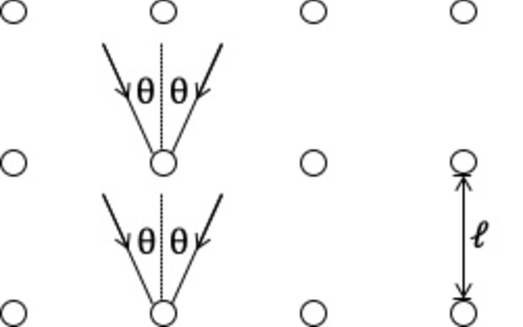
\includegraphics[width=100mm]{images/quantum/dgschem.pdf}
\end{figure}

Each layer of the crystal has an electron beam hitting it and bouncing off at about the same angle. If we believe that electrons are waves, they will interfere. This is because they travel different distances to get to the same point. Constructive interference will occur when the waves are exactly in phase, meaning when the difference in the paths traveled by beams hitting different layers is a multiple of the wavelength. Since the difference in path length between the layers of the crystal is $\Delta l =2l \sin \theta$, as you can see from the figure, this means that constructive interference occurs when $\Delta l = n \lambda$ for integral $n$. 

Davisson and Germer did actually observe an interference pattern as predicted by our theory. By measuring the angles at which constructive interference occurred, they could calculate a wavelength for the electron beam, which they found to be equal to $\tfrac{h}{p}$, where $h$ is Planck's constant and $p$ is the electrons' momentum. This gives us the equation for the de Broglie wavelength $\lambda = \tfrac{h}{p}$.

The phenomenon Davisson and Germer demonstrated is now called \textbf{Bragg scattering}. It can be used to calculate the lattice spacing of a crystal by shining an electron beam or light beam of known wavelength upon it and measuring the angles at which constructive interference is found. For the discovery of matter waves, Davisson received the Nobel Prize in Physics in 1937 (Germer was only nominated).

\subsection{Conclusions}
These experiments, as well as some others (including the double-slit experiment), implied that electrons and photons act both as particles and as waves. Other experimental results, such as the spectrum of hydrogen, could also not be explained with classical mechanics. A new formulation of physics was needed, and quantum mechanics developed to explain all of these strange results. 